\section{Introduction}
This project describes a~selected \textit{operational research} problem according to the~particular published research paper~\cite{paper}.
A~given problem is defined in Chapter~\ref{sec:problem}.
Approaches to a~solution to the~problem from the~paper are re-implemented,~and experimental results are finally compared with the~results in the~paper and with the~student results from the~previous years.

The~rest of this documentation is organised as follows.
Chapter~\ref{sec:method} presents an~approach to the~solution to the~problem,~and there are also described appropriate methods.
Re-implementation of the method is then depicted in Chapter~\ref{sec:implementation}.
Experimental evaluation is discussed in Chapter~\ref{sec:experiments}.
Finally,~Chapter~\ref{sec:conclusion} concludes this documentation and achieved project results.

\section{University Course Timetabling Problem} \label{sec:problem}
\textit{University Course Timetabling Problem} (\textit{UCTP}) is known as an~\emph{NP-hard} problem.
It is defined as a~set of rooms,~events in the~schedule,~students and room features,~the~completion of which individual courses require.
The UCTP solution is then assigned free room and item in the~time-schedule for each of a~given number of courses for meeting all the~specified features and conditions.
In more precise,~an~UCTP is an~optimisation problem that deals with the~scheduling process. 
The~aim is to find such a~distribution of the course into classrooms and schedule times,~which does not conflict with \textit{hard} constraints,~and at the~same has the~lowest possible score of \textit{soft} constraints.
Since this is a~problem that is often solved and analyzed in practice,~there are already countless methods used in implementing the~solution.
The~categories into which the~ways of solving optimisation problems can be divided are from the~various areas.
It is often a~method of \textit{simulated annealing},~the~application of \textit{genetic algorithms},~or generally inspired by \textit{nature},~such as optimising \textit{ants colonies} and last but not least \textit{genetic algorithms}.

\subsection{Formal Definition}
An instance of the UCT problem is defined as follows:
\begin{itemize}
    \item A set of $N$ courses, $e = \{ e_1, \dots, e_N\}$
    \item $45$ time-slots
    \item A set of $R$ rooms
    \item A set of $F$ room features
    \item A set of $S$ students
\end{itemize}
where tor each room,~its capacity and the~features it provides are also given. 
For each student,~there is a~list of subjects to be enrolled in,~and for each course,~lists the~required features.
Further, this problem includes $4$ \textit{hard} constraints and $3$ \textit{soft} constraints as follows.
\paragraph{Hard Constraints:}
\begin{itemize}
    \item \textbf{Event Conflict} ($H_1$): no student can be assigned to more than one course at the~same time
    \item \textbf{Room Features} ($H_2$): the~room should satisfy the~features required by the~event
    \item \textbf{Room Capacity} ($H_3$): the~number of students attending the~event should be less than or equal to the~room capacity
    \item \textbf{Room Occupancy} ($H_4$): no more than one event is allowed at a time slot in each room
\end{itemize}
\paragraph{Soft Constraints:}
\begin{itemize}
    \item \textbf{Event in the Last Time Slot} ($S_1$): a~student shall not have to attend a~course that is scheduled in the~last time slot of the~day
    \item \textbf{Two Consecutive Events} ($S_2$): a~student shall not have more than two consecutive events
    \item \textbf{One Event a Day} ($S_3$): a~student shall not have to attend a~single course on a~day
\end{itemize}
Once the~solution of the~UCTP instance is found,~it is first assessed in terms of meeting the~inviolable (\textit{hard}) constraints.
If it does not conflict with any of these hard restrictions,~the~solution is marked as \textit{feasible},~so it is a~valid and usable solution.
Violent (\textit{soft}) constraints are then used to assess and compare the~quality of the actual results.
The~lower the~value of the~conflict with these constraints for the~given solution,~the higher the~quality of the~solution.
For \textit{genetic} algorithms,~this \textit{score} represents the~value of the~fitness function of a~given solution - the \textit{chromosome}.
This fitness function for the problem is defined in the
formula below
\begin{align*}
    \min \sum_{s=1}^{S}{s_1 + s_2 + s_3}
\end{align*}
where $s_1$, $s_2$ and $s_3$ represents the relevant soft constraints score individually for each student.

\section{Differential Evolution Algorithm} \label{sec:method}
The~proposed method is named \textit{Differential Evolution Algorithm}, which is based on the~principle of \textit{genetic algorithms},~but unlike them,~the~key operation is not a~\textit{cross} but a~\textit{mutation}.
The~implemented method can be logically divided into two phases. 
In the~first part,~an~initial population is created,~representing a~set of valid schedules,~and then a~\textit{Differential Evolution Algorithm} is applied. 
An~algorithm that aims to increase the~quality of the~solution while maintaining the~integrity of all inviolable (hard) constraints.

\subsection{Constructive Heuristic} \label{sec:const}
The first step of the~algorithm is creating the~\textit{initial population},~i.e. the~production of a~given number of \textit{chromosomes},~each of which represents a~valid solution of the~specified UCTP instance.
Creating one schedule consists of the~gradual assignment of rooms and part of the schedule to each of the~courses.
To increase the~success of this initial creation,~the~courses are first sorted according to the~number of rooms to which they can be assigned \,--\, which is determined based on the~capacity of the~room and its features.
Subsequently,~the~sorted courses are placed in the~schedule gradually from those to which the~smallest number of rooms can be assigned.
We note,~that in this process,~the~soft restrictions are not taken into account at all in this process.
When a~\textit{feasible} solution can be created in this way,~the current \textit{chromosome} is added to the~\textit{population}, and the~algorithm continues to create a~new solution or by moving to the~second part of the~algorithm.

Otherwise,~when the~algorithm gets into a~situation where there is no free time and room for the~currently placed course,~the~\textit{neighbourhood moves} are applied to the~yet placed courses.
The aim is to rearrange the finished part of the~schedule to free space for the~currently placed course.
First,~the~\textit{neighbourhood move} $N_1$ is performed several times. The algorithm continues by placing the~current course when the~schedule was successfully rearranged.
Otherwise,~the \textit{neighbourhood move} $N_2$ is performed repeatedly.
If it is still not possible to find a~place for the~currently placed course,~the~placement of the~following courses is continued.
The~different neighbourhood structures and their explanation can be outlined as follows:

\paragraph{Neighbourhood Move $N_1$.}
Choose a~single course at random and move to a~feasible time slot that can generate the~lowest penalty cost.

\paragraph{Neighbourhood Move $N_2$.}
Select two courses at random from the~same room (the room is randomly selected) and swap time slots.

\noindent\\
The~technique described above should lead to one valid solution to the~problem. 
When the current schedule cannot be successfully filled, this solution is removed from the~\textit{population}.

\subsection{Improvement Algorithm}
Once the~complete initial population is generated,~the~second phase of the~whole algorithm can begin,~which is the~optimisation by the~\textit{evolutionary algorithm}.
\textit{Genetic algorithms} inspire the implemented differential evolution algorithm,~and its main emphasis is on \textit{mutation} operations.
One iteration of the~described algorithm consists of four parts:~\textit{mutations}, \textit{crossover},~\textit{evaluation},~and \textit{selection}.
This sequence of steps is applied repeatedly until at least one of the~terminating conditions is reached.
These are the~achievement of a~fixed number of iterations (generations) or the~acquisition of a~solution whose value of the~fitness function is equal to 0.
The~base schema of this algorithm is presented below:

\begin{align*}
    & Initialisation \\
    & Evaluation \\
    & \textbf{do while} \; (termination \; criteria \; are \; met) \\
    & \quad Mutation \\
    & \quad Crossover \\
    & \quad Evaluation \\
    & \quad Selection \\
    & \textbf{end do while}
\end{align*}

\begingroup\vspace*{-\baselineskip}
\captionof{figure}{Differential Evolution Algorithm.}
\vspace*{\baselineskip}\endgroup

\paragraph{Mutation.}
The~\textit{mutation} is a central part of the~implemented differential evolution algorithm.
The~first step of the~mutation is the~random selection of two parental chromosomes \,--\, i.e. two complete solutions \,--\, from the~population.
Then a~mutation is performed by selecting one of the~two mutation operators and then applying it to each of the~parents separately.
Mutation operators are the~same as neighbourhood moves described in Section~\ref{sec:const}.
This results in a~modified pair of \textit{parental chromosomes}.

\paragraph{Crossover.}
Crossover is an~operation whose purpose is to generate two new descendants.
The~input of this operation is two-parent chromosomes obtained by mutation operation.
For each parent,~one time is randomly generated in the~schedule,~and in the~parent chromosomes,~the courses planned for a~given time are interchanged.
In order to maintain the~validity of the~solution in the~offspring,~two conditions are placed on the~exchange of the~course.
The~course can be moved only if it is free in the~second schedule on the~moving position, and moving the course to a~new location will not cause any collisions between courses.

\paragraph{Evaluation and Selection.}
Evaluation is used to evaluate newly born offspring.
To evaluate each of the~offspring,~a \textit{fitness function} is used,~which calculates a~penalty for non-compliance with violable (\textit{soft}) restrictions.
If a~better offspring has a~lower value of \textit{fitness function} than the~best individual in the~population so far,~the worst-rated chromosome in the~population is replaced by the~better of the~offspring.

\section{Implementation} \label{sec:implementation}
The described algorithm has been implemented in Python programming language.
At least,~it is required Python version 3.6.
Python libraries NumPy\footnote{Python library for mathematics computation
NumPy\,--\,\url{https://numpy.org}.} and SciPy\footnote{Python library
for mathematics computation SciPy\,--\,\url{https://www.scipy.org}.} was used for mathematics computation and work with series and lists.
Required versions of these libraries,~as well as the~next needed libraries,~are specified in the~file \texttt{requirements.txt}.
The~implementation consists of several modules described in the~paragraphs below.

\noindent \\
The module \texttt{ucctp.py} severs an~entry point of the application.
It sets a~routine for logging,~parses arguments from the~command line and calls the~main function of the~whole application.
The module \texttt{input.py} reads and validates an input file with the specification of the problem.
It contains functions for reading and parsing input files with the~specification of the~problem,~and function for writing solutions to output file in the~appropriate format.

\noindent\\
A~class \texttt{UcctpInstance} represents the~University Course Timetabling Problem.
This class encapsulates the~specification of the~problem as well as its input parameters.
Moreover, it contains operations over the problem instance that cannot be derived directly from input data.
For instance,~there is implemented the~method for sorting the~events according to the~number of rooms which they can be assigned,~the~method for computing the~collision events,~so events that have one or more common students,~or the~method to compute available rooms for courses,~and some other auxiliary methods.

\noindent\\
The most interesting is module \texttt{differential\_e\-volution.py} which contains main functions.
The method \texttt{run} serves as the~wrapper over the~whole algorithm,~and it gradually performs all required operations.
Firstly,~it loads and parses the algorithm parameters from the~file \texttt{parameters.json} and save them into the~relevant program structure.
The~next step is to create an~initial population of the chromosomes. 

This is done using the~\texttt{constructive\_heuri\-stics} method,~which creates a~population of the required size by repeatedly calling the~\texttt{construct\_e\-vent\_time\-table} method.
In the~way described above tries to place all the~courses one after the~other and thus create a~complete schedule. 
If there is nowhere to place a~course,~the already mentioned neighbourhood moves are applied. 
In particular,~the~\texttt{apply\_mo\-ve\_n1} and \texttt{apply\_move\_n2} methods are used for this purpose.
The~chromosomes that are not complete,~i.e. even after the~application of neighbourhood moves,~no suitable location was found for any course,~are not appended to the~population.
Moreover,~as the~fulfilment of inviolable constraints is che\-cked already during the~creation of the~schedule,~we do not have to incorrectly remove chromosomes after generation.

Subsequently,~the~\texttt{evaluate\_timetables} me\-thod calculates the~evaluation of all chromosomes in a~population-based on how much they do not satisfy the~violation (soft) constraints. 
The \texttt{object\_func\-tion} method is implemented to calculate the penalty for violating restrictions $s_1$, $s_2$ and $s_3$.
The~quality of each individual is then given as the~sum of these three values. 
According to the~evaluation of individual chromosomes,~the~entire population is sorted from the~highest quality to the~lowest quality in the~same method (\texttt{evaluate\_timetables}).

Now the~differential evolution algorithm itself can begin. 
Until the~specified number of iterations is exceeded,~or the~best solution in the~population does not have a~zero value of the~fitness function,~the \texttt{differe\-ntial\_evolution\_algorithm} method is repeatedly called,~which performs one iteration implemented algorithm.
Thus,~the~\texttt{mutation} and \texttt{crossover} methods are gradually performed. 
Then,~the~evaluation is performed,~and if one of the~offspring represents a~better solution than the best one so far,~the~new offspring replaces the~worst solution in the~population.

\subsection{Algorithm Enhancement}
The implementation of the~original algorithm often had a~problem finding a~\textit{feasible} solution.
Moreover,~the~paper does not contain a~strictly detailed description of how the~creation of the~original population should take place.
As a~result,~there was space in this area for change and improved the~existing algorithm.

The~placement of the~course is still gradual from the~most problematic one.
For the~selection of the room and the~time slot until which the~course will be filled,~we implemented the~\texttt{get\_timetable} method, which selects the~most suitable of all available locations.
In more precise,~the~method \texttt{get\_final\_ti\-metable} first selects the~most suitable time slots,~wh\-ich are the~ones in which there are already the~most occupied rooms.
The~reason is that such time slots will be the~hardest to fill in the~future,~as there is a~high probability that a~conflict rate will already be located here.
Therefore,~all possible course locations are limited to those that take place in the~most appropriate time slots selected.

Subsequently,~from the~remaining locations,~the~on\-es that take place in the~most suitable rooms are selected by the~\texttt{get\_final\_time\-table} method.
Th\-ese are the~rooms in which the~smallest number of courses that have not yet been filled can be placed. 
Here the reason is clear,~again the~aim is to provide as many opportunities as possible for further courses.
From these locations that meet the~above conditions for both the~room and the~time slot is then randomly selected as the~final location.

\section{Experimental Evaluation} \label{sec:experiments}
The~reference to the~set of tests on which the~original implementation was tested is no longer functional and could not be traced on other servers.
However,~we found the GitHub repository\footnote{\url{https://github.com/tomas-muller/cpsolver-itc2007}} which contains the International Timetabling Competition data-sets.
From this data set,~we took a~set of instances with a~similar structure to the~one in the~original paper.
As well as the~original set,~the~new one contains a~total of 11 tests,~of which 5 correspond to the~specification of small test input,~the~other 5 are medium and 1 input problem falls into the~category of large inputs.
A~description of the~properties that the~input file of a~given size meets is given in the~following table:
\begin{table}[ht!]
\centering
\begin{tabular}{|l|c|c|c|}
\hline
\textbf{Category} & \multicolumn{1}{l|}{\textbf{Small}} & \multicolumn{1}{l|}{\textbf{Medium}} & \multicolumn{1}{l|}{\textbf{Large}} \\ \hline
\textbf{N (courses)}        & 100                                 & 300-400                              & 400                                 \\ \hline
\textbf{R (rooms)}        & 5                                   & 10                                   & 10                                  \\ \hline
\textbf{F (features)}        & 5                                   & 5                                    & 10                                  \\ \hline
\textbf{S (students)}        & 80                                  & 200                                  & 200                                 \\ \hline
\textbf{max N per S}  & 20                                  & 20                                   & 20                                  \\ \hline
\textbf{max S per N}  & 20                                  & 50                                   & 100                                 \\ \hline
\textbf{max F per R}  & 3                                   & 3                                    & 5                                   \\ \hline
\textbf{\% usage of F}     & 70                                  & 80                                   & 90                                  \\ \hline
\end{tabular}
\caption{Description of the properties of individual categories of test inputs.}
\end{table}

To mimic the~experiments performed in the~original paper as much as possible,~all arguments were set to the~same values when experimenting as in the~original experiments performed by the~paper authors.
An overview of the parameters values used is as follows:
\begin{lstlisting}[language=json,firstnumber=1]
{
    "generations_number": 200000,
    "population_size": 50,
    "crossover_rate": 0.8,
    "mutation_rate": 0.5,
    "n1_applications": 100,
    "n2_applications": 100
}
\end{lstlisting}

\begin{table*}[ht!]
\begin{center}
\begin{tabular}{|l|c|c|c|c|c|c|}
\hline
\textbf{Input}   & \multicolumn{1}{l|}{\textbf{Paper}} & \multicolumn{1}{l|}{\textbf{xvitra00}} & \multicolumn{1}{l|}{\textbf{xmarus06}} & \multicolumn{1}{l|}{\textbf{xvales03}} & \multicolumn{1}{l|}{\textbf{xvales02}} & \multicolumn{1}{l|}{\textbf{xstupi00}} \\ \hline
\textbf{small1}  & 0                                   & \textbf{11}                            & 33                                     & 31.2                                   & 47                                     & 42                                     \\ \hline
\textbf{small2}  & 0                                   & 21                                     & 32                                     & 34.5                                   & 21                                     & \textbf{20}                            \\ \hline
\textbf{small3}  & 0                                   & \textbf{16}                            & 26                                     & 28.0                                   & 38                                     & 25                                     \\ \hline
\textbf{small4}  & 0                                   & 45                                     & 42                                     & \textbf{41.7}                          & 53                                     & 46                                     \\ \hline
\textbf{small5}  & 0                                   & \textbf{20}                            & 30                                     & 32.5                                   & 37                                     & 27                                     \\ \hline
\textbf{medium1} & 160                                 & \textbf{27}                            & 234                                    & 255.9                                  & 237                                    & 198                                    \\ \hline
\textbf{medium2} & 81                                  & 154                                    & 132                                    & 126.2                                  & \textbf{62}                            & 71                                     \\ \hline
\textbf{medium3} & 149                                 & \textbf{117}                           & 269                                    & 289.8                                  & 205                                    & 230                                    \\ \hline
\textbf{medium4} & 113                                 & \textbf{26}                            & 170                                    & 173.1                                  & 66                                     & 51                                     \\ \hline
\textbf{medium5} & 143                                 & \textbf{27}                            & 145                                    & 168.2                                  & 76                                     & 59                                     \\ \hline
\textbf{large}   & 735                                 & 369                                    & 468                                    & 408.4                                  & 342                                    & \textit{\textbf{325}}                  \\ \hline
\end{tabular}
\caption{Comparison of various algorithms on the individual input instances.}
\label{tab:compare}
\end{center}
\end{table*}

\subsection{Results Comparison}
As in the~original experiments,~a~total of 11 times were tested for each test problem,~and the~lowest value of the~result was always selected for this report.
Due to the absence of the~original set,~the~results of the~implementation were compared with the~implementations of the~algorithms implemented by the students in the previous years, which are available in their GitHub pages\footnote{\url{https://github.com/marusak/UCTPS/blob/master/doc.pdf}}\footnote{\url{https://github.com/Bihanojko/SNT/blob/master/doc.pdf}}.
A~comparison of the algorithms on the~
individual test inputs is given in Table~\ref{tab:compare}.
For each input instance of the~problem,~the~best of the~achieved values is marked here in bold,~i.e.~the~algorithm that achieved the~best solution on the~given input.
The~implemented algorithm achieved two times the~best result. 
On the~contrary,~only in one case,~it turned out the~worst at all,~so it is a~competitive algorithm.
We note, that the~\textit{xvales02} implements the~same method as we.
Compared with the~original implementation,~Table~\ref{tab:compare} also shows the~values obtained by the authors of the original paper. 
However,~this comparison is not very meaningful,~as the~input instances correspond in size,~but still be one-sided problems and values of the~best possible solutions can vary considerably.

\subsection{Influence of population-size parameter}
The~next part of the~experimenting deals with examining the~influence of the~value of the~\textit{population-size} parameter on the~population's quality.
This parameter certainly affects the~value of the~\textit{fitness function} of the~solution,~the~larger the~original population,~the~more parent chromosomes can be selected for crossbreeding,~and thus the~more diverse chromosomes we can obtain.
For each input set,~experiments were performed with a~\textit{population size} ranging from 10 to 100 individuals with a~step of 10.
The~number of generations was always set to 100 so that the~iterative increase in population quality was not reflected too much in the~results of the~experiment.
The~resulting characteristics for each of the 11 test inputs are shown in Figures~\ref{fig:smallp},~\ref{fig:mediump},~\ref{fig:largep}.
From the ~graphs,~it is clear that randomness greatly influences the~quality of the~population. 
Still,~when looking at the~whole curve,~the~expected hypothesis is confirmed: The~greater the~number of individuals in the~population,~the higher the~quality of the~population.

\subsection{Influence of generations-number parameter}
The~last part of the~experiments is devoted to examining the effect of the~\textit{generations-count} parameter on the~quality of the~resulting solution.
This parameter significantly affects the~value of the~\textit{fitness function} of the~result,~as the~population can improve in each generation.
Its research can also be useful if we would like to use the~application for quality calculations in the~shortest possible time because,~for a~higher number of generations,~the~calculation time starts to increase significantly.
For each input set,~the~experiment has performed 10 times,~and then the~run that achieved the~greatest improvement over the~generations was plotted.
The~experiments were performed with a~population size of 50 individuals,~and the~quality of the~population was recorded in the~range from 0 to 20000 generations with step 1. 
The~values of the~graph were obtained in an~excerpt from the application after each iteration.
The~resulting characteristics for each of the~11 test inputs are shown in Figure~\ref{fig:smallg},~\ref{fig:mediumg},~\ref{fig:largeg}. 
There is a~clear improvement in all cases,~with a~near logarithmic decrease at the~beginning of the~curve,~and later primarily a~linear.

\noindent \\
These~experiments confirmed both the~correctness of the~re-implementation of the~algorithm and the~functionality and efficiency of the~original algorithm.

\begin{figure*}[h]
\centering
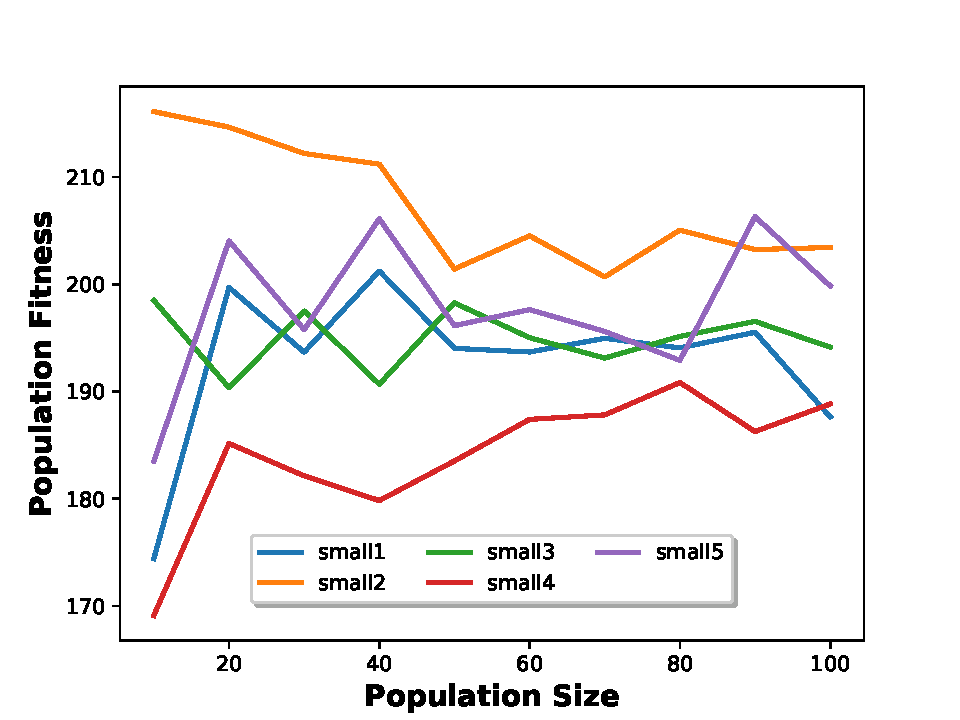
\includegraphics[height=0.30\textheight]{figures/small_population.pdf}
\caption{Influence of population-size parameter for small problem instances.}%
\label{fig:smallp}%
\end{figure*}

\begin{figure*}[h]
\centering
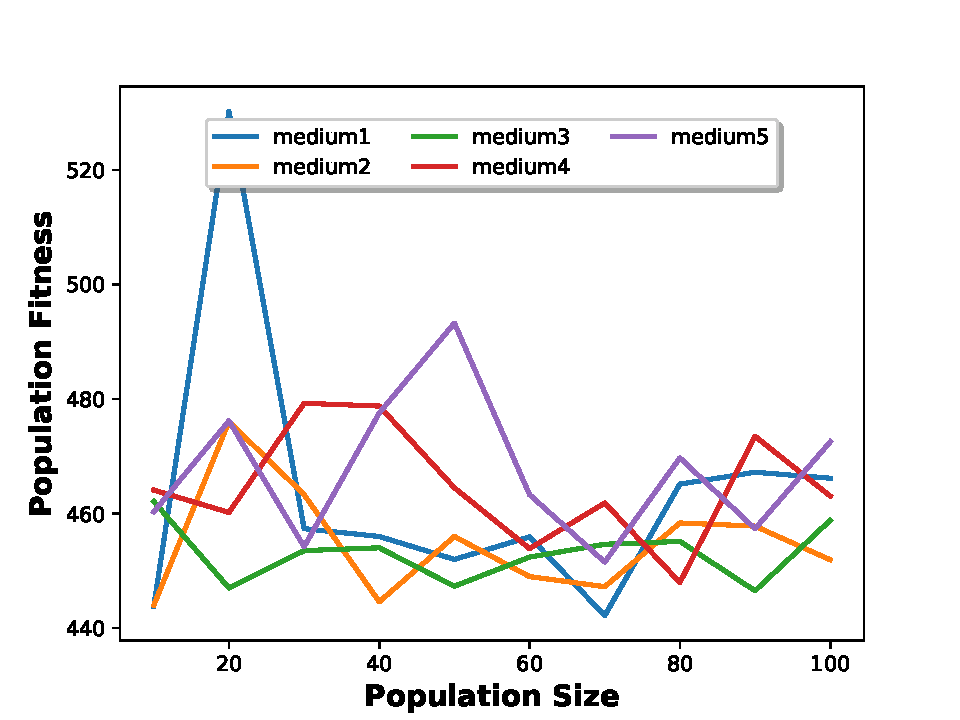
\includegraphics[height=0.30\textheight]{figures/medium_population.pdf}
\caption{Influence of population-size parameter for medium problem instances.}%
\label{fig:mediump}%
\end{figure*}

\begin{figure*}[h]
\centering
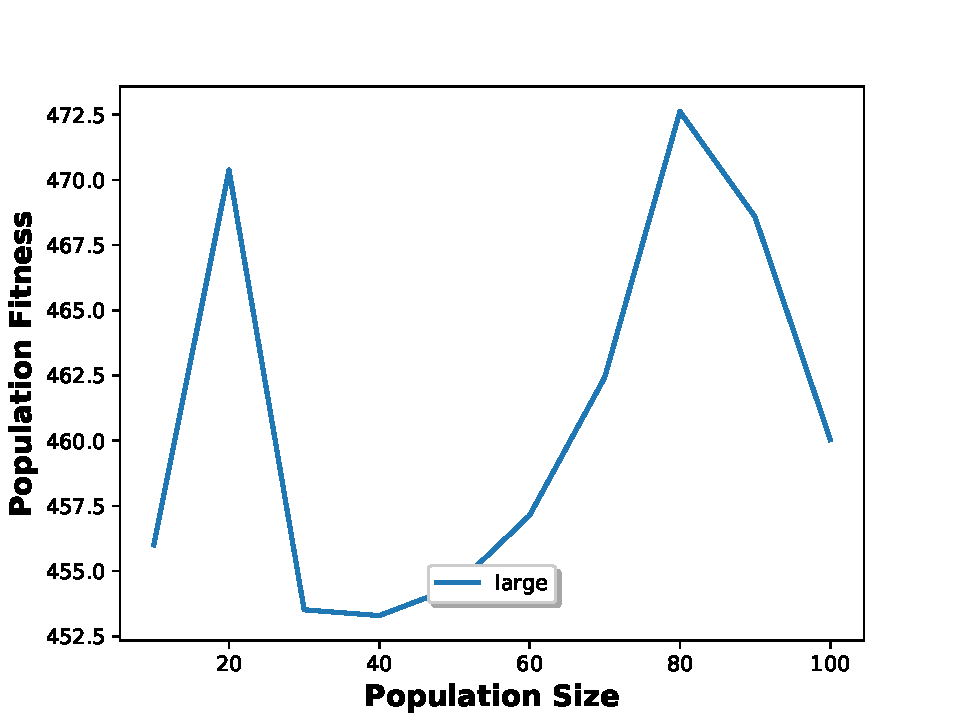
\includegraphics[height=0.30\textheight]{figures/large_population.pdf}
\caption{Influence of population-size parameter for large problem instance.}%
\label{fig:largep}%
\end{figure*}

\begin{figure*}[h]
\centering
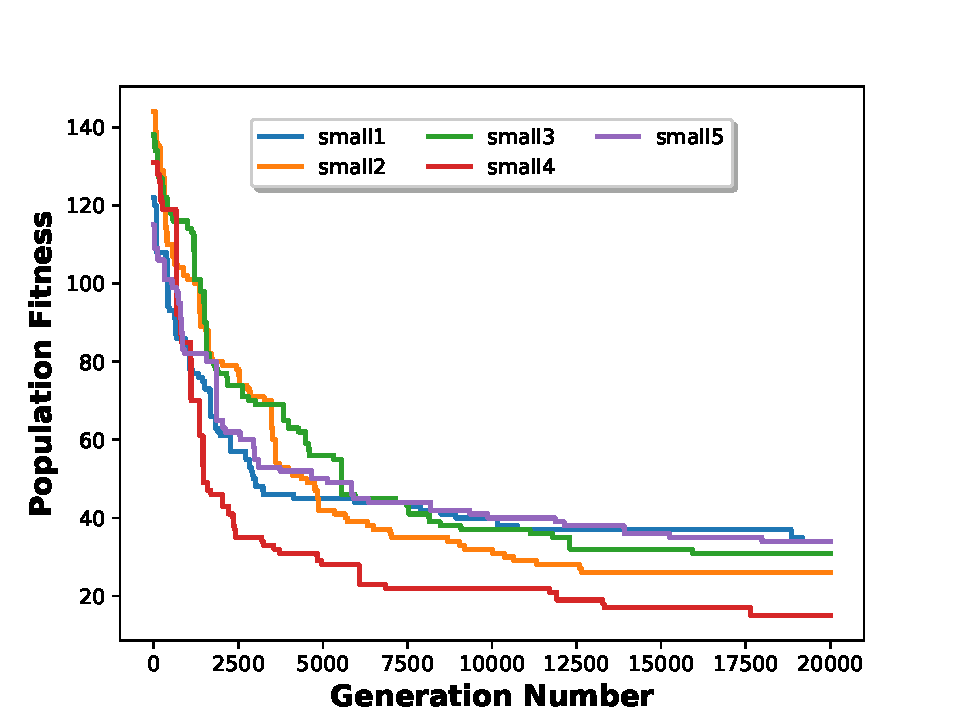
\includegraphics[height=0.30\textheight]{figures/small_generation.pdf}
\caption{Influence of generations-number parameter for small problem instances.}%
\label{fig:smallg}%
\end{figure*}

\begin{figure*}[h]
\centering
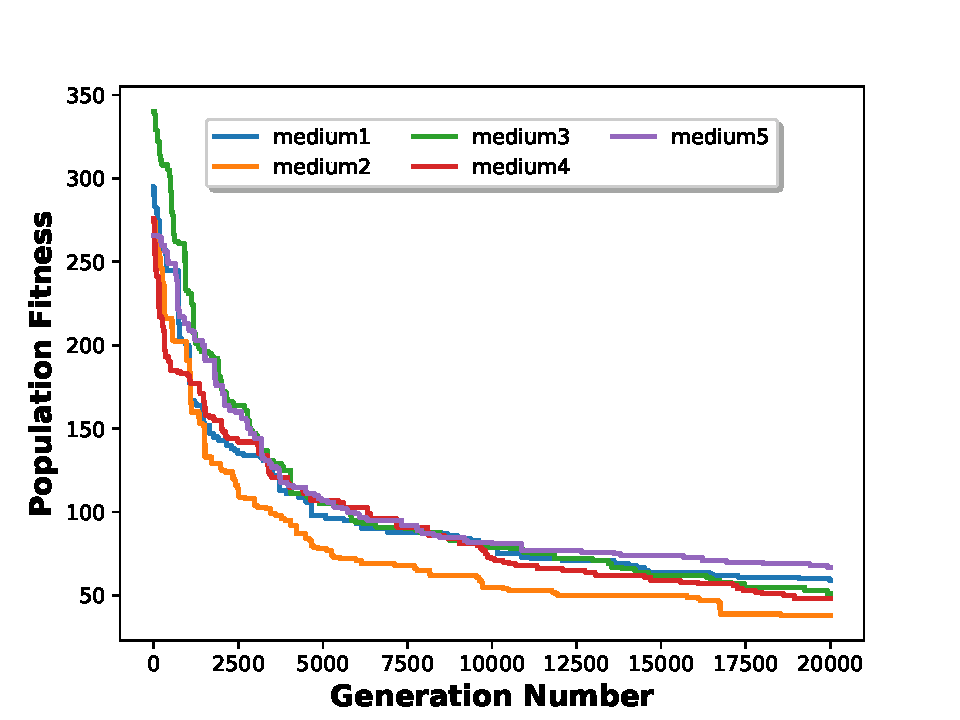
\includegraphics[height=0.30\textheight]{figures/medium_generation.pdf}
\caption{Influence of generations-number parameter for medium problem instances.}%
\label{fig:mediumg}%
\end{figure*}

\begin{figure*}[h]
\centering
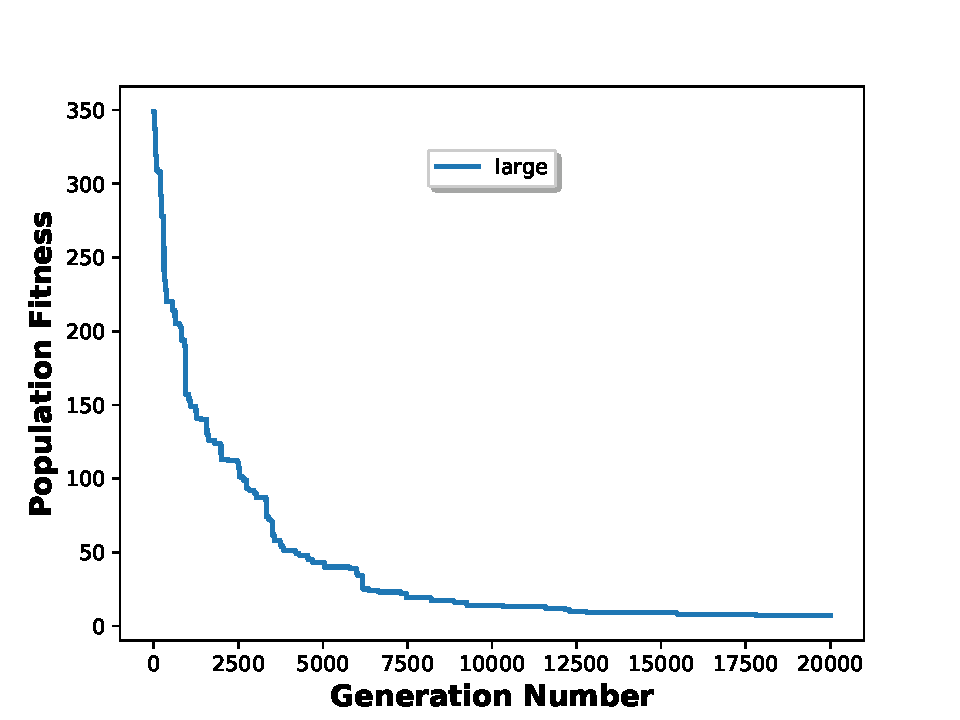
\includegraphics[height=0.30\textheight]{figures/large_generation.pdf}
\caption{Influence of generations-number parameter for large problem instance.}%
\label{fig:largeg}%
\end{figure*}

\section{Conclusion} \label{sec:conclusion}

As part of this project,~an~algorithm called \textit{Differential Evolution Algorithm} was studied and re-implemented.
Subsequently,~several experiments were performed with the~implementation,~comparing this approach with other algorithms,~examining the~effect of population size on the~quality of solutions,~and the~number of generations on the~quality of the~total population.
The~functionality of the~re-implementation was verified by these experiments.